\documentclass{../res/univ-projet}

%Import des packages utilisés pour le document
\usepackage[utf8x]{inputenc}
\usepackage[francais]{babel}
\usepackage[T1]{fontenc}
%\usepackage{array}
%\usepackage{hyperref}
%\usepackage{tabularx, longtable}
%\usepackage[table]{xcolor}
%\usepackage{fancyhdr}
%\usepackage{lastpage}

\definecolor{gris}{rgb}{0.95, 0.95, 0.95}

%Redéfinition des marges
%\addtolength{\hoffset}{-2cm}
%\addtolength{\textwidth}{4cm}
\addtolength{\topmargin}{-1cm}
\addtolength{\textheight}{1cm}
\addtolength{\headsep}{0.8cm} 
\addtolength{\footskip}{-0.2cm}


%Import page de garde et structures pour la gestion de projet
%\usepackage{structures}

%Variables
\logo{../res/logo_univ.png}
\title{Spécification Technique de Besoin}
\author{Ibrahima-Sory \bsc{Barry}, Bertille \bsc{Bouillie}}
\projet{GPG}
\projdesc{Interface Graphique GPG}
\filiere{M1SSI - Conduite de Projet}
\version{0.1}
\relecteur{Olivier \bsc{Thibault}}
\signataire{Magali \bsc{Bardet}}
\date{\today}

\histentry{0.3}{17/11/2014}{Ajout des modifications demandées par le client.}
\histentry{0.2}{09/11/2014}{Ajout des exigences.}
\histentry{0.1}{31/10/2014}{Version initiale.}

% -- Début du document -- %
\begin{document}

%Page de garde
\maketitle
\newpage
%La table des matières
\tableofcontents
\newpage

\section{Objet}

% Présentation succinte du sujet et hyp de travail.
Ce document est la Spécification Technique du Besoin de la réalisation d'une interface graphique pour le logiciel GnuPG.

\subsection{Besoins opérationnels}
\begin{itemize}
 \item Accès à toutes les fonctionnalités de GnuPG.
 \item Utilisation pédagogique et précise : l'interface doit permettre à toute personne novice en sécurité d'utiliser l'application, et une aide doit être donnée pour chaque action.
\end{itemize}

\subsection{Objectifs techniques}
\begin{itemize}
 \item Gestion fine des clés : choix de la taille, de l'algrithme de chiffrement symétrique.
 \item Gestion et aperçu de la toile de confiance.
 \item Chiffrement et déchiffrement pour le webmailing.
 \item Visualisation de la ou des lignes de commande GnuPG équivalentes pour chaque action lancée.
\end{itemize}

\subsection{Contraintes et recommandations}
\begin{itemize}
 \item L'application doit fonctionner sur le système d'exploitation GNU/Linux, en particulier, sous les environnements KDE et Gnome.
\end{itemize}

\subsection{Résultats attendus}
\begin{itemize}
 \item Rapport complet de l'étude de GnuPG : liste de toutes les fonctionnalités.
 \item Implémentation d'une interface graphique pour toutes les fonctionnalités de GnuPG.
 \item Document d'explications et de recommandations à l'utilisation de l'interface graphique.
 \item Document d'analyse des limites cryptographiques de PGP.
 \item Implémentation de l'attaque sur les KeyId décite dans l'article «Surveillance généralisée : aux limites de PGP» du numéro 75 du magazine MISC.
\end{itemize}



\section{Documents applicables et de référence}
% Liste des
% - Références des documents quidefinissent formellement les principes
%   directeurs et le hypothèse de travail prise en compte pour l'établissement de la spécification.
% - Références des documents cités dans la STB au titre d'explication ou de justification.
Différents documents de référence :
\begin{itemize}
\item Définitions du standard OpenPGP \href{file:../../ressources/openPGP/rfc4880-en.pdf}{RFC 4880}
  et \href{file:../../ressources/openPGP/rfc2440-fr.pdf}{RFC 2440}
\item Le logiciel \href{https://www.gnupg.org/}{GnuPG} (GNU Privacy Guard) implantation Open Source
  de OpenPGP.
\item La \href{https://www.gnupg.org/gph/fr/manual.html#AEN541}{toile de confiance} de GnuPG
\item Editeurs graphiques existant 
  (\href{http://www.gnupg.org/related_software/frontends.en.html}{KGpg, GPA, Seahorse})
\item Exemple de visualisation d'une toile de confiance sur le site de 
  \href{https://www.archlinux.org/master-keys/#visualization}{archlinux}.
\end{itemize}

%\section{Terminologie et sigles utilisés}
%\textcolor{blue}{
 % \begin{itemize}
  %\item Glossaire ou dictionnaire
  %\item Abréviations
  %\item Formalisme utilisé
  %\item Légendes et conventions de représentation
  %\end{itemize}
%}

\section{Exigences fonctionnelles}
\subsection{Présentation de la mission du produit logiciel}

\begin{tabular}{|>{\centering}p{1cm}|>{\centering}p{7cm}|>{\centering}p{2.5cm}|>{\centering}p{3cm}|}
  \hline
  \color{white}\cellcolor{blue}\bfseries{Id}&
  \color{white}\cellcolor{blue}\bfseries{Intitulé}&
  \color{white}\cellcolor{blue}\bfseries{Acteur(s)}&
  \color{white}\cellcolor{blue}\bfseries{Priorité}\\
  \cr
  \hline
  EF\_1&
  Exécution d'actions GPG&
  Utilisateur&
  Indispensable
  \cr
  \hline
  EF\_2&
  Chiffrement/déchiffrement, signature/vérification&
  Utilisateur&
  Indispensable
  \cr
  \hline
  EF\_3&
  Affichage des commandes, des retours et des erreurs&
  Utilisateur&
  Indispensable
  \cr
  \hline
  EF\_4&
  Choix du profil&
  Utilisateur&
  Indispensable
  \cr
  \hline
  EF\_5&
  Modification de la toile de confiance graphique&
  Utilisateur&
  Important
  \cr
  \hline
  EF\_6&
  Création de clé d'attaque sur les KeyId&
  Utilisateur&
  Indispensable
  \cr
  \hline
\end{tabular}\\

\newpage

%Cas d'utilisation
\subsection{Interface graphique}

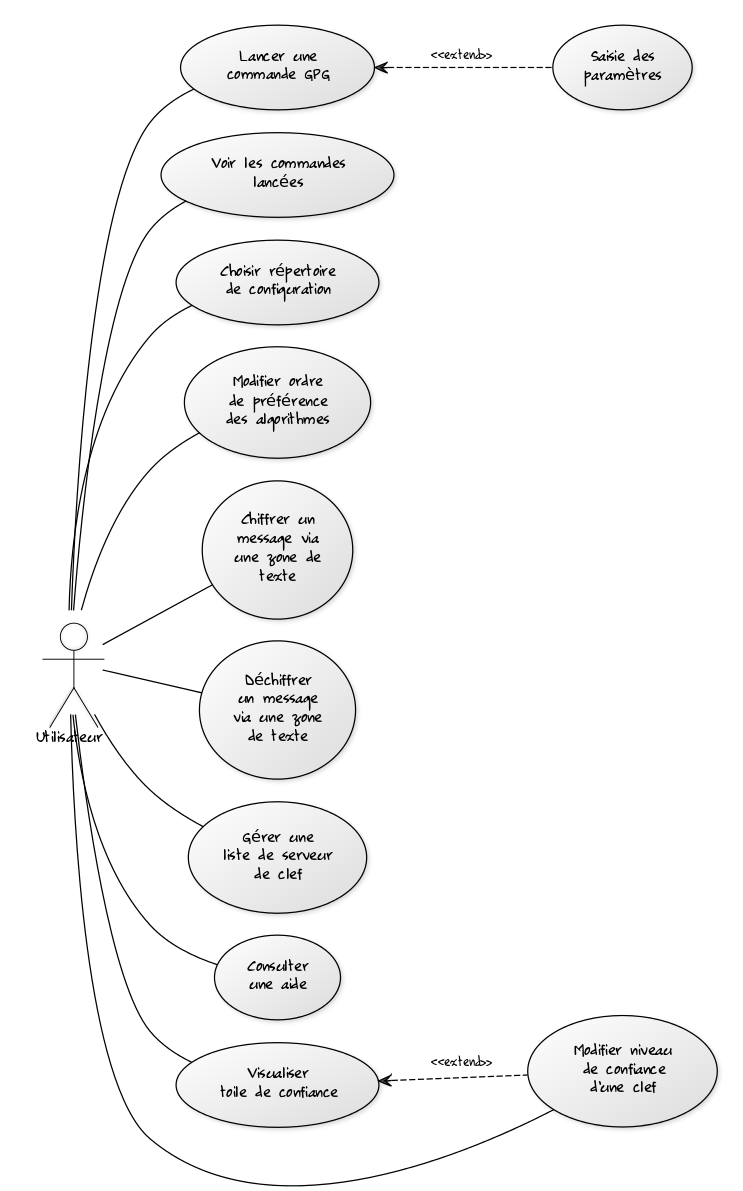
\includegraphics[scale=0.5]{../res/graphics/Diag_utilisation}
  \subsubsection{Cas d'utilisation 1}
\ficheGraphic
% Nom du cas d'utilisation
{Exécution d'actions GPG}
% Acteurs concernés
{Utilisateur}
% Description
{
  Fonctionnement du système pour chaques actions
  necessitant l'intervention de GPG.
  Toutes ces actions sont spécifiée dans les
  \newline
  \href{file:../../ressources/openPGP/rfc4880-en.pdf}{RFC 4880}
  et \href{file:../../ressources/openPGP/rfc2440-fr.pdf}{RFC 2440}
}
% Préconditions
{}
% Evénements déclenchants
{Demande d'action GPG}
% Conditions d'arrêt
{Action terminée}
% Diagramme
{0.5}{../res/graphics/Diag_Seq_Actions_GPG_v2}
% Flots d'exceptions
{
  \begin{itemize}
  \item Abandon de l'utilisateur.
  \item Erreurs GPG.
  \end{itemize}
}
% Fin de la fiche du cas d'utilisation 1.
\vspace{0.5cm}

  \subsubsection{Cas d'utilisation 2}
\ficheGraphic
% Nom du cas d'utilisation
{Chiffrement/déchiffrement, signature/vérification}
% Acteurs concernés
{Utilisateur}
% Description
{Chiffrement ou déchiffrement du ou des fichiers sélectionnés, ou du texte copié dans l'éditeur de l'interface, selon le choix de l'utilisateur. Signature ou vérification d'un document.}
% Préconditions
{Pour un chiffrement et une signature, l'utilisateur possède une clé. Pour un déchiffrement et une vérification, l'utilisateur possède la clé public dans son trousseau.}
% Evénements déclenchants
{Demande de chiffrement, déchiffrement, signature ou vérification.}
% Conditions d'arrêt
{}
% Diagramme
{0.5}{../res/graphics/Diag_Seq_Chiff_Dechiff_v2}
% Flots d'exceptions
{Abandon de l'utilisateur.}
% Fin de la fiche du cas d'utilisation 2.
\vspace{0.5cm}

  \subsubsection{Cas d'utilisation 3}
\ficheGraphic
% Nom du cas d'utilisation
{Affichage des commandes, des retours et des erreurs}
% Acteurs concernés
{Utilisateur}
% Description
{L'utilisateur peut choisir d'afficher ou non les commandes, les retours et les erreurs, associées à chaque action GPG.}
% Préconditions
{}
% Evénements déclenchants
{Demande de modification de l'affichage.}
% Conditions d'arrêt
{}
% Diagramme
{0.5}{../res/graphics/Diag_Seq_Affichage_Commandes_v2}
% Flots d'exceptions
{}   
% Fin de la fiche du cas d'utilisation 3.
\vspace{0.5cm}

  \subsubsection{Cas d'utilisation 4}
\ficheGraphic
% Nom du cas d'utilisation
{Choix du profil}
% Acteurs concernés
{Utilisateur}
% Description
{L'utilisateur peut modifier le profil à l'ouverture grâce à l'option -P, ou à tout autre moment. Si au démarrage, l'option -P n'est pas précisée, et qu'aucun profil par défaut n'est défini, l'utilisateur doit choisir un profil.}
% Préconditions
{}
% Evénements déclenchants
{Ouverture avec l'option -P, ouverture sans profil par défaut, ou demande de modification du profil par l'utilisateur.}
% Conditions d'arrêt
{}
% Diagramme
{0.5}{../res/graphics/Diag_Seq_Config}
% Flots d'exceptions
{Abandon de l'utilisateur.}
% Fin de la fiche du cas d'utilisation 4.
\vspace{0.5cm}

Le fichier de configuration de l'interface contient les différents profils, ainsi que le profil par défaut. Chaque profil possède un répertoire GPG.



  \subsubsection{Cas d'utilisation 5}
\ficheGraphic
% Nom du cas d'utilisation
{Modification de la toile de confiance graphique}         
% Acteurs concernés
{Utilisateur}
% Description
{Modification de la Toile de confiance, par un changement de niveau de confiance ou l'ajout d'un nouveau membre, via la représentation graphique de la toile.}
% Préconditions
{La représentation de la toile de confiance doit apparaître à l'écran.}
% Evénements déclenchants
{Demande de modifications par l'utilisateur.}
% Conditions d'arrêt
{Sauvegarde et mise à jour de l'affichage terminées.}
% Diagramme
{0.5}{../res/graphics/Diag_Seq_Toile}
% Flots d'exceptions
{Abandon de l'utilisateur.}                      
% Fin de la fiche du cas d'utilisation 5.
\vspace{0.5cm}
  

\subsection{Implémentation de l'attaque sur les KeyId}
  
  \subsubsection{Cas d'utilisation 6}
\ficheGraphic
% Nom du cas d'utilisation
{Création de clé d'attaque sur les KeyId}
% Acteurs concernés
{Utilisateur}
% Description
{Création d'une clé d'attaque à partir d'une clé publique, selon la méthode décrite dans le numéro 75 du MISC.}
% Préconditions
{L'utilisateur doit être en possession d'une clé publique.}
% Evénements déclenchants
{Demande de création de clé d'attaque.}
% Conditions d'arrêt
{Clé d'attaque créée.}
% Diagramme
{0.5}{../res/graphics/Diag_Seq_Attaque}
% Flots d'exceptions
{}
% Fin de la fiche du cas d'utilisation 6.
\vspace{0.5cm}
  
\newpage

\section{Exigences opérationnelles}

\begin{tabular}{|>{\centering}p{1,5cm}|>{\centering}p{10cm}|>{\centering}p{3cm}|}
  \hline
  \color{white}\cellcolor{blue}\bfseries{Id}&
  \color{white}\cellcolor{blue}\bfseries{Intitulé}&
  \color{white}\cellcolor{blue}\bfseries{Priorité}\\
  \cr
  \hline
  EO\_1&
  Implémentation GnuPG 2.0.*&
  Indispensable
  \cr
  \hline
  EO\_2&
  Implémentation GnuPG 1.4.*&
  Optionnel
  \cr
  \hline
  EO\_3&
  Fonctionnement sous KDE 4.*&
  Indispensable
  \cr
  \hline
  EO\_4&
  Fonctionnement sous Gnome 3.*&
  Important
  \cr
  \hline
  EO\_5&
  Fonctionnement sous Windows 7 et 8&
  Optionnel
  \cr
  \hline
  EO\_6&
  Représentation graphique de la Toile de confiance&
  Indispensable
  \cr
  \hline
  E0\_7&
  Ouverture de deux interfaces avec des profils différents sur une même session&
  Important
  \cr
  \hline
  EO\_8&
  Connexion SSH : Authentification par clé signée par GPG&
  Optionnel
  \cr
  \hline
\end{tabular}\\



\section{Exigences opérationnelles d'interface}

Le client n'a aucune exigence opérationnelle d'interface.


\section{Exigences de qualité}

\begin{tabular}{|>{\centering}p{1,5cm}|>{\centering}p{10cm}|>{\centering}p{3cm}|}
  \hline
  \color{white}\cellcolor{blue}\bfseries{Id}&
  \color{white}\cellcolor{blue}\bfseries{Intitulé}&
  \color{white}\cellcolor{blue}\bfseries{Priorité}\\
  \cr
  \hline
  EQ\_1&
  Représentation des niveaux de confiance par couleurs sur la liste des clés&
  Important
  \cr
  \hline
  EQ\_2&
  Temps de réponse et fluidité de l'interface&
  Indispensable
  \cr
  \hline
  EQ\_3&
  Interface livrée sous forme de paquet Ubuntu&
  Optionnel
  \cr
  \hline
\end{tabular}\\

\section{Exigences de réalisation}

Le client n'a aucune exigence de réalisation.

%\begin{tabular}{|>{\centering}p{1,5cm}|>{\centering}p{10cm}|>{\centering}p{3cm}|}
%  \hline
%  \color{white}\cellcolor{blue}\bfseries{Id}&
%  \color{white}\cellcolor{blue}\bfseries{Intitulé}&
%  \color{white}\cellcolor{blue}\bfseries{Priorité}\\
%  \cr
%  \hline
%\end{tabular}\\

\end{document}

